\section{Evaluation}
\label{sec:eval}

We evaluate \sys{} across six single-variable hardware campaigns
(\textbf{E1--E6}) totaling \textbf{1,723 verified runs} ($n=3$ interleaved
repetitions per point, plus $n=5$ for key credit-off controls in E6; medians
reported). Every process binds to Socket~1 memory (\texttt{numactl --membind=1})
with \texttt{mlockall}. Every accepted run passes automated gates: zero packet
corruption/tearing (header/mid/trailer checks), zero credit-line tearing, zero
measurement-window page faults, 100.00\% non-multiplexed host and SmartNIC PMUs,
zero PAUSE frames, and zero post-campaign host/card EDAC or PCIe AER increments
after a 21--22\,s settle window. All retries (e.g., transient clock droop or
cable PHY CRC) are logged without silent omission.

\subsection{E1: Unfenced Credit Cost, Safety Cliff, and Pause Ablation}
\label{sec:eval-e1}

\begin{figure*}[t]
  \centering
  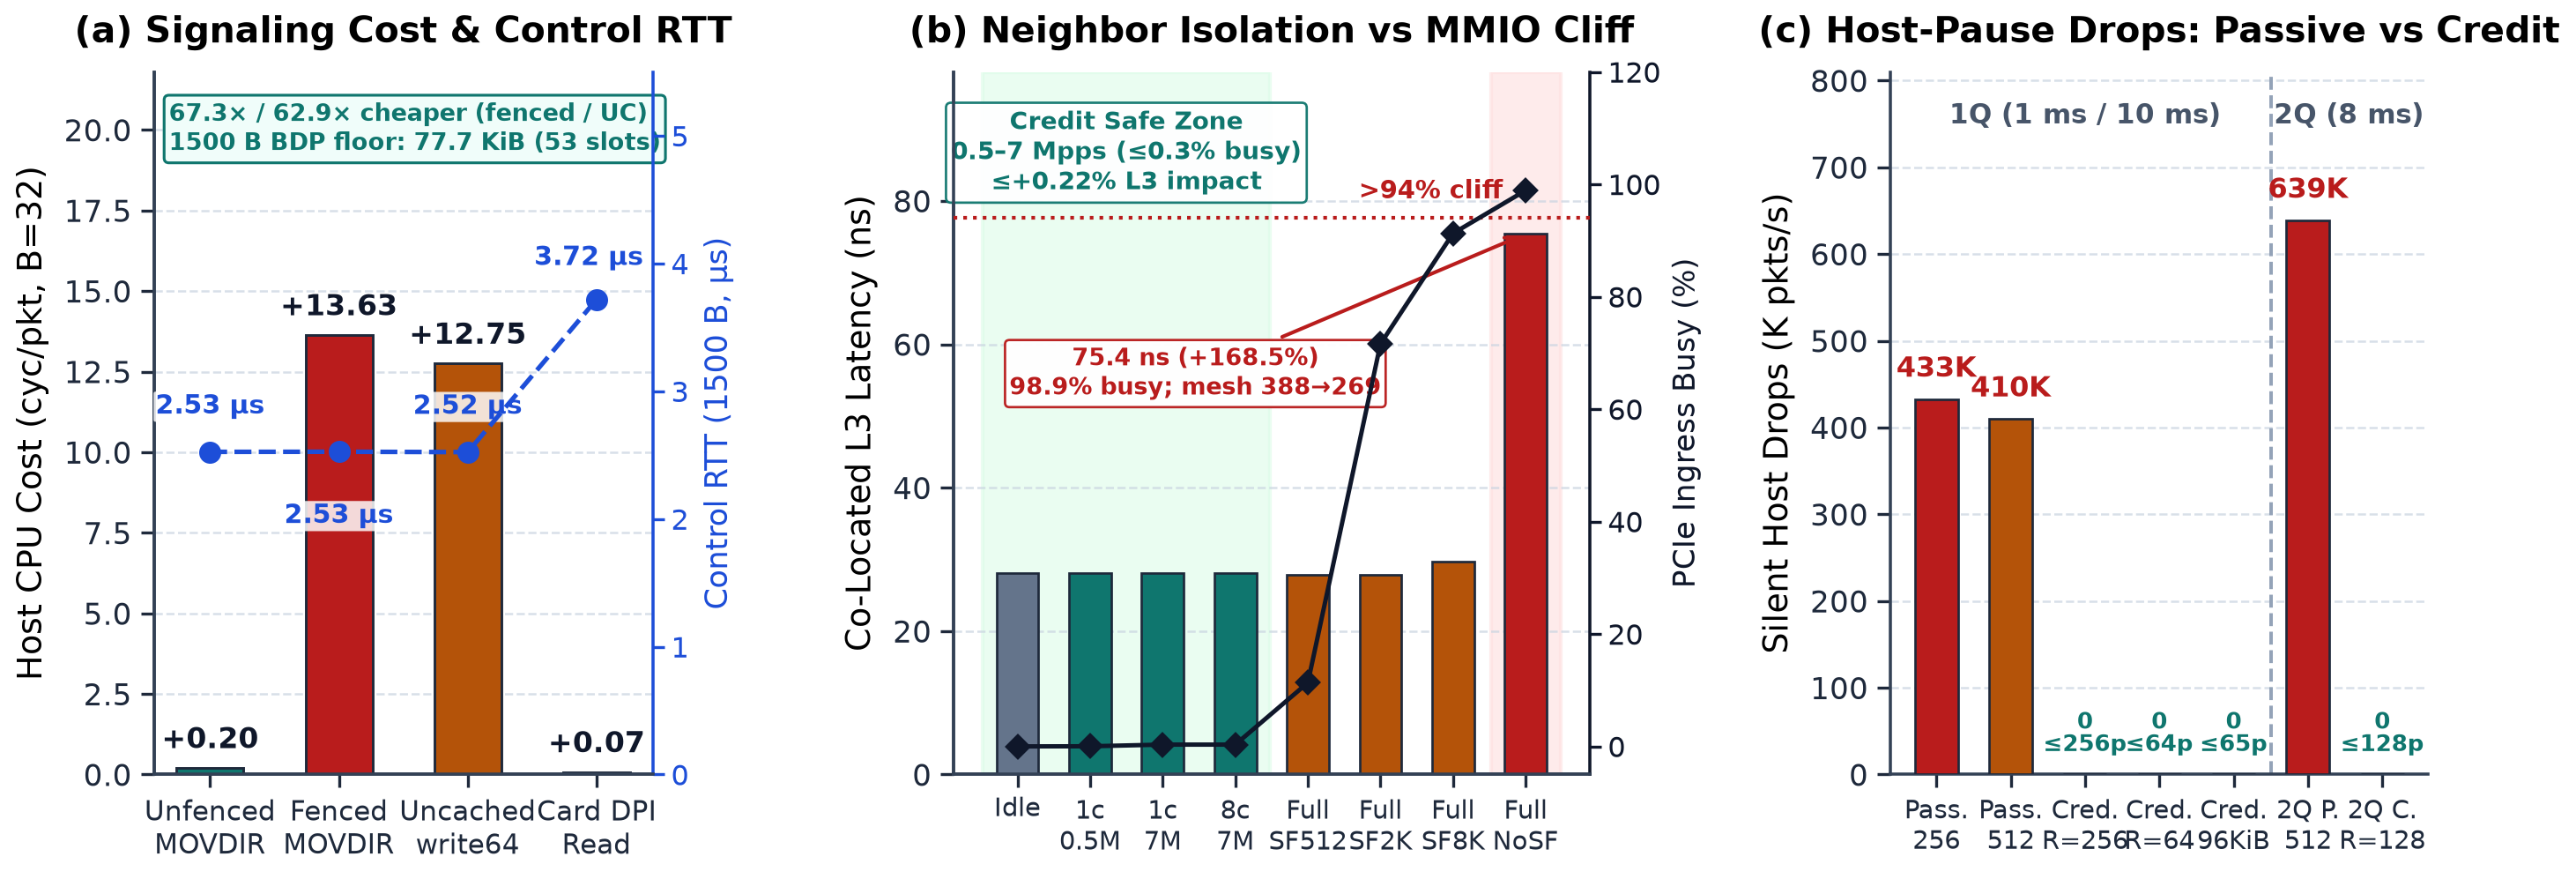
\includegraphics[width=\textwidth]{figures/fig2_e1_signaling.png}
  \caption{\textbf{E1 (354 runs, 618M pkts):} Unfenced BAR4 MMIO credit
  microbenchmarks. (a)~Unfenced \texttt{MOVDIR64B} adds +0.20 host cyc/pkt at
  $B=32$ (67.3$\times$/62.9$\times$ cheaper than fenced/UC) with 2.53\,$\mu$s
  control RTT. (b)~Real credit rates (0.5--7\,Mpps, 1--8 cores) cause
  $\le$+0.22\% L3 impact, while unconstrained flooding ($\sim$175\,Mpps)
  crosses the $>$94\% PCIe ingress cliff (+168.5\% L3 latency even as aggregate
  mesh occupancy falls). (c)~Explicit BAR4 credits cut 410K--639K silent
  passive-SDP pause drops to zero with exact packet/byte residency caps.}
  \label{fig:e1}
\end{figure*}

Figure~\ref{fig:e1} summarizes 354 verified runs (618M packets) isolating
unfenced 64-byte BAR4 credit signaling.

\paragraph{CPU cost, unloaded latency, and descriptor-slot BDP.}
Matching real $B=32$ batch spacing ($\sim$168\,ns/batch, Figure~\ref{fig:e1}(a)),
unfenced \texttt{MOVDIR64B} adds just \textbf{+6.48 cycles/batch (+0.20 cyc/pkt)}
with 0.01 cycles/batch store-buffer stalls, versus \textbf{+436.25 cycles/batch
(+13.63 cyc/pkt, 67.3$\times$)} with \texttt{SFENCE} and \textbf{+408.00
cycles/batch (+12.75 cyc/pkt, 62.9$\times$)} for uncached 64-bit writes
($>$97\% store-buffer stalls). Compressing writes to the same BAR4 line down to
$\sim$15\,ns hits Sapphire Rapids same-line mesh serialization (112.9\,ns/batch),
motivating $B \ge 16$--$32$ batching. On unloaded $W=1$ ping-pong ($B=32$),
unfenced credits add only \textbf{+5.4 to +16.3\,ns} median latency (+10.6 to
+19.1\,ns full-loop $1/\text{rate}$).

Closed-loop control RTT (\texttt{ism\_enable=1}) is \textbf{2.12--2.15\,$\mu$s}
(64\,B) and \textbf{2.52--2.53\,$\mu$s} (1500\,B) across all BAR4 modes, beating
SmartNIC DMA host-memory reads (3.25 / 3.72\,$\mu$s) by \textbf{1.10--1.19\,$\mu$s}.
By Eq.~\ref{eq:bdp-slots} ($B=32$), 1500\,B at 100GbE (8.22\,Mpps) requires
only \textbf{$\sim$53 slots / 77.7\,KiB} wire bytes (77.3\,KiB payload;
106\,KiB of 2\,KiB \texttt{mbuf}s), giving 128--256-slot hot rings
2.4--4.8$\times$ slot headroom (3.3--6.6$\times$ payload headroom). Conversely,
64\,B at 90--148.8\,Mpps demands \textbf{226--353 descriptor slots}
(452--706\,KiB of 2\,KiB \texttt{mbuf}s), underscoring why descriptor-slot BDP
governs small-packet ring sizing.

\paragraph{Neighbor zero-interference boundary vs.\ $>$94\% PCIe cliff.}
Across 0.5--7.0\,Mpps unfenced credit rates (1, 4, and 8 cores,
Figure~\ref{fig:e1}(b)), co-located 16\,MiB L3 latency stays at
\textbf{28.00--28.15\,ns} vs.\ 28.08\,ns idle ($\le +0.22\%$) and 6-core STREAM
Triad stays at \textbf{49.82--50.16\,GB/s} vs.\ 49.99\,GB/s ($\le \pm 0.35\%$),
with PCIe ingress busy $\le 0.3\%$ and aggregate mesh occupancy $\le 2.8$. By
contrast, driving a single core at unconstrained $\sim$175.3\,Mpps and stepping
periodic fences down (\texttt{SF512} $\to$ \texttt{SF2048} $\to$ \texttt{SF8192}
$\to$ none) pushes PCIe ingress busy to \textbf{98.9\%}---past the
\textbf{$>$94\% zero-drain cliff}---spiking L3 latency by \textbf{+168.5\%}
(28.1 $\to$ 75.4\,ns; $K=32$ $p99$ to 216\,ns) and cutting 6-core STREAM
bandwidth by \textbf{$-$25.0\%} (50.0 $\to$ 37.5\,GB/s at 92.7\% ingress busy;
$-$5.7\% already at \texttt{SF8192} / 86.6\%), even while aggregate mesh
occupancy counter-intuitively \emph{drops} from 387.6 to 268.5 (522.4 $\to$
364.7 under STREAM). Sustained PCIe ingress occupancy is thus the governing
congestion metric, proving why unfenced MMIO belongs strictly on low-rate
credit signaling.

\paragraph{Data safety and passive-SDP pause ablation.}
Across 617.5M full-rate packets (103.71\,Gbps on 1500\,B, 25.81\,Mpps on 64\,B),
static in-place rings (100.00\% IOVA stability) and dynamic poisoned
\texttt{mbuf} replacement (0.03--0.64\% IOVA stability, both $B=64$ and
unaligned $B=32$) record zero corruption, tearing, or reordering under
Eq.~\ref{eq:wmark-invariant}. During periodic 1\,ms/10\,ms host pauses (1500\,B
at 5\,Mpps, Figure~\ref{fig:e1}(c)), CN106's default passive SDP rings (256 /
512 slots, \texttt{SDPX\_OUT\_BP\_ENX\_W1S = 0}) silently drop \textbf{432.9K /
410.1K} packets/s (1.31--1.34M/s on 64\,B at 15\,Mpps; \textbf{639.1K}/s on
paused Q1 during 8\,ms 2Q stalls) while card FIFO stays at $\le 32$. Explicit
BAR4 credits eliminate all drops (\textbf{0}) across every packet ($R=256, 128, 64$)
and byte (96\,KiB, 8\,KiB) window, bound residency exactly, and losslessly
absorb an unscheduled 1.95\,ms host preemption (5,666 packets).

\subsection{E2: 100GbE Burst Protection and Line-Rate Net Draining}
\label{sec:eval-e2}

\begin{figure*}[t]
  \centering
  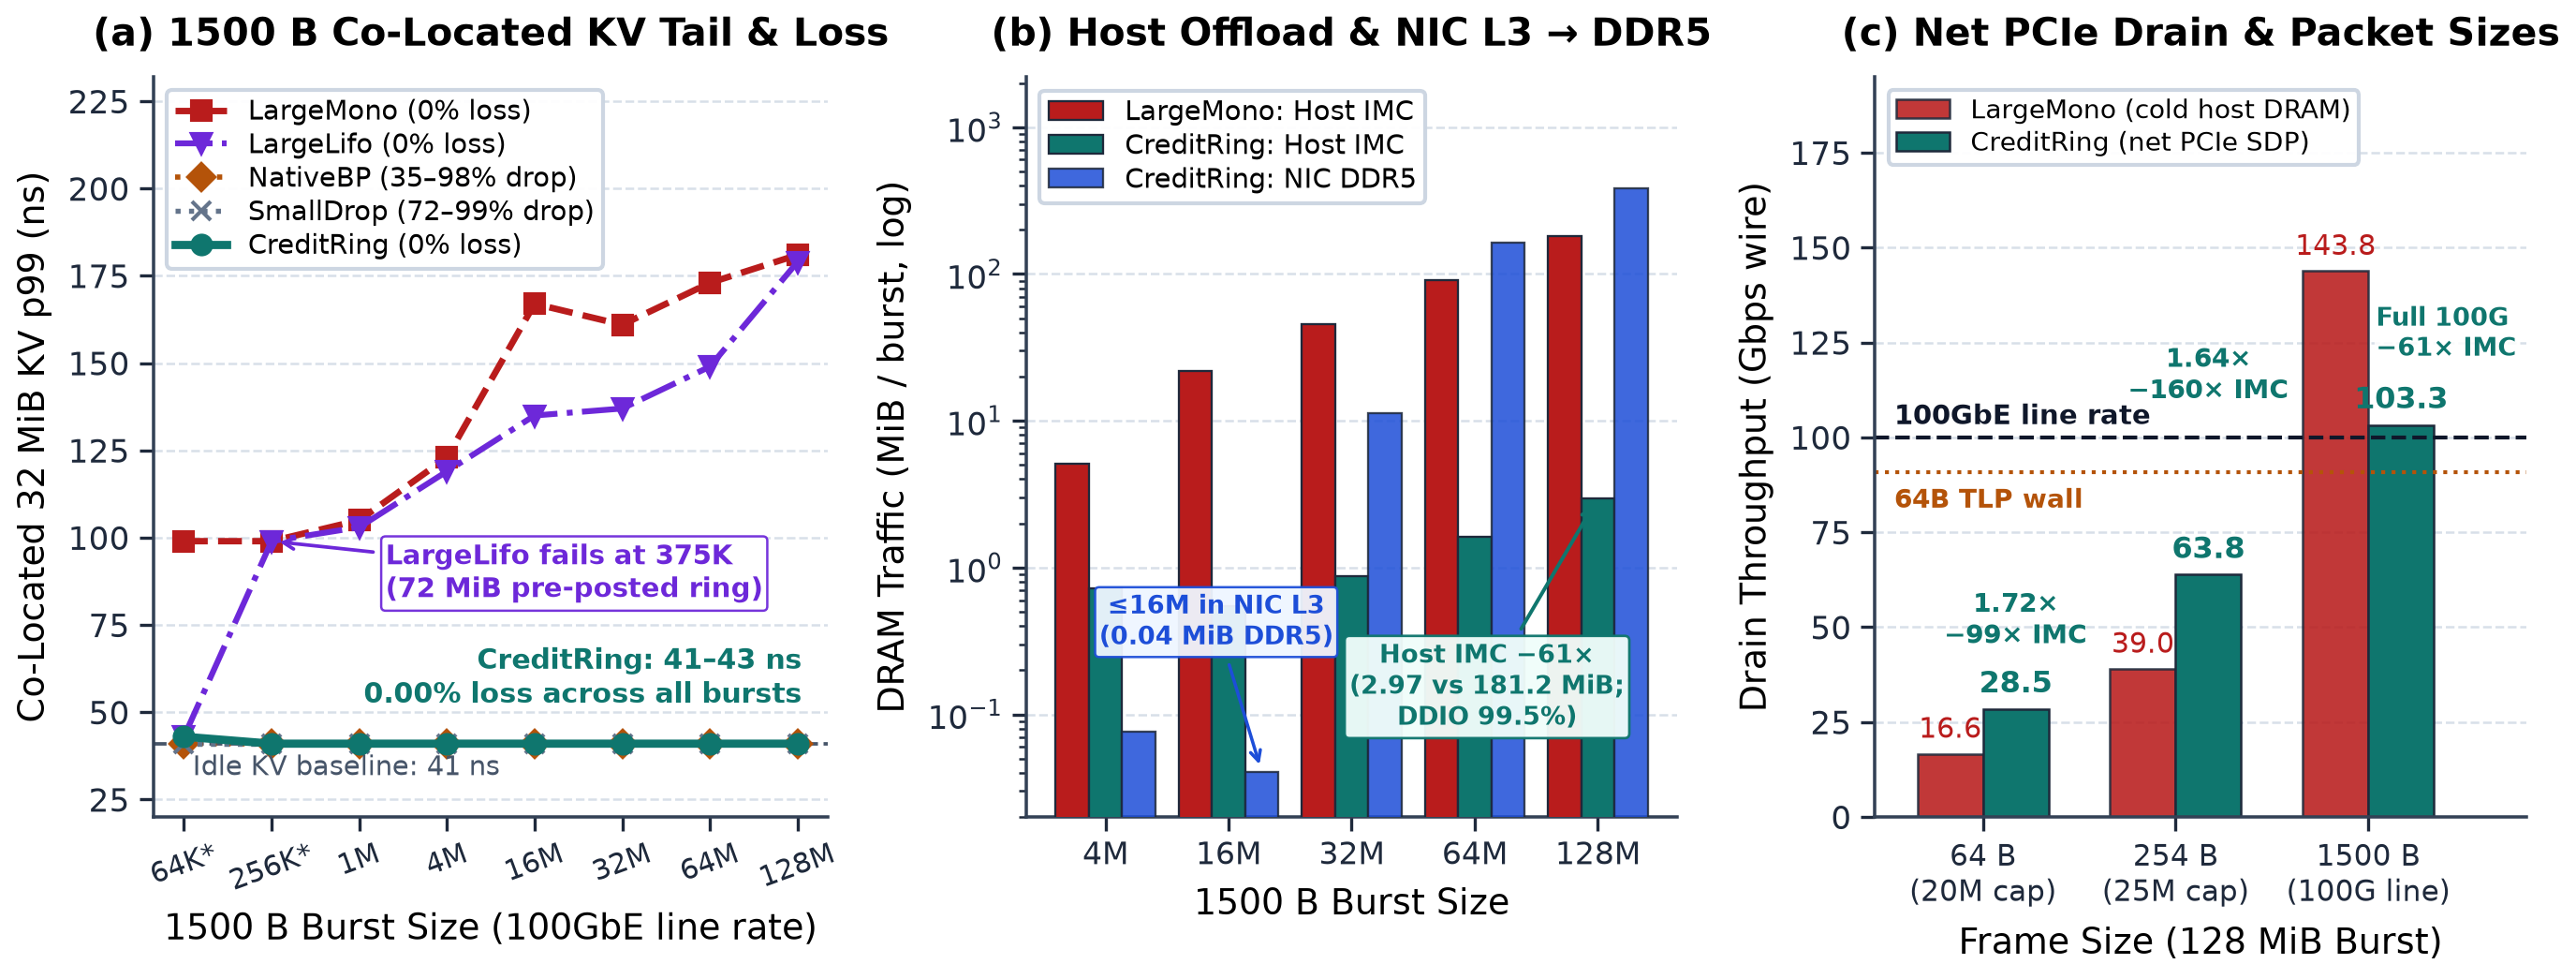
\includegraphics[width=\textwidth]{figures/fig3_e2_burst_100g.png}
  \caption{\textbf{E2 (393 runs, 534M pkts):} Real 100GbE + standard SDP bursts
  (64\,KiB--128\,MiB) with a co-located 32\,MiB KV workload. (a)~At 1500\,B line
  rate, only \sys{} sustains 0.00\% loss and 41--43\,ns idle KV $p99$;
  \texttt{LargeLifo} fails even at 375\,KiB due to the 72\,MiB pre-posted ring.
  (b)~Host DRAM traffic drops 61$\times$ at 128\,MiB (99.5\% DDIO), with
  $\le$16\,MiB bursts absorbed in SmartNIC L3 (0.04\,MiB card DDR5) and larger
  bursts offloaded to card 6-ch DDR5. (c)~Net PCIe SDP drain reaches 103.3\,Gbps
  wire-equivalent on 1500\,B and beats cold 2-channel host DRAM by
  1.64--1.72$\times$ on 254\,B / 64\,B (99--160$\times$ less host IMC).}
  \label{fig:e2}
\end{figure*}

Figure~\ref{fig:e2} spans 393 verified runs (534M packets) across 64\,B, 254\,B,
and 1500\,B bursts (64\,KiB--128\,MiB; 1500\,B 64/256\,KiB align to 256 packets
= 375\,KiB L2, marked `*'; 64\,B / 254\,B paced at 20 / 25\,Mpps for lossless
single-core large-ring baselines) alongside a co-located 32\,MiB KV workload
(idle $p50=31$\,ns, $p99=41$\,ns, $p999=97$\,ns).

\paragraph{Burst isolation and the pre-posted ring bound.}
At 1500\,B 100GbE (Figure~\ref{fig:e2}(a)), \texttt{SmallDrop} (256 slots) and
\texttt{NativeBP} (512 slots) silently drop \textbf{71.6--99.1\%} and
\textbf{35.2--98.0\%} for bursts $\ge 4$\,MiB. Large host rings
(\texttt{LargeMono}, \texttt{LargeLifo}, using a software host backlog during
arrival) avoid loss but inflate KV $p99$ \textbf{4.4$\times$} to
\textbf{181 / 179\,ns} ($p999 = 293$\,ns, L3 miss 17.7--17.8\%) at 128\,MiB.
Even at 375\,KiB and 1\,MiB, \texttt{LargeLifo} collapses to 2.0--4.5\% DDIO
(KV $p99$ 99--103\,ns), confirming Eq.~\ref{eq:fifo-lower-bound}: four
pre-posted 8192-slot rings span 72.0\,MiB ($>60$\,MiB LLC), whereas smaller
254\,B / 64\,B rings (20 / 12\,MiB) hold 74--96\% DDIO until bursts exceed
32,768 packets. Only \sys{} achieves \textbf{0.00\% loss} across all bursts
(buffering 88,576 packets at 128\,MiB) while locking KV $p99$ at
\textbf{41.0--43.0\,ns} (0.60\% L3 miss) and DDIO at \textbf{98.1--99.5\%}.

\paragraph{Memory offload and line-rate net PCIe draining.}
At 128\,MiB (1500\,B, Figure~\ref{fig:e2}(b)), \sys{} slashes host DRAM traffic
\textbf{61.0$\times$} (181.20 $\to$ 2.97\,MiB/burst, $-98.4\%$). SmartNIC PMUs
verify clean two-tier offloading: $\le 16$\,MiB stays inside CN106's 48\,MiB L3
(\textbf{0.04\,MiB/burst} card DDR5), 32\,MiB spills lightly (11.27\,MiB), and
64--128\,MiB drains smoothly through 6-channel card DDR5 (163.2 / 383.9\,MiB).

Subtracting the 1,024 hot-ring packets pre-delivered before drain starts
(which make raw apparent drain read 150.3 $\to$ 104.5\,Gbps), true \textbf{net
PCIe SDP draining} (\texttt{fifo\_deq / drain\_s}) converges to
\textbf{95.7 $\to$ 102.2 $\to$ 102.9 $\to$ 103.0 $\to$ 103.3\,Gbps} wire rate
across 4--128\,MiB (16--128\,MiB marginal slope \textbf{103.45\,Gbps} wire /
102.09\,Gbps L2). Host inbound PCIe writes reach \textbf{12.95\,GB/s}
(12.81\,GB/s net), surpassing the 11.46\,GB/s (90.9\,Gbps) 64\,B TLP wall via
standard large-TLP DMA within the 126.03\,Gbps physical Gen5~$\times 4$ limit.

On 254\,B and 64\,B at 128\,MiB (Figure~\ref{fig:e2}(c)), large rings sweep
632.6 / 2,049.7\,MiB/burst of host DRAM (partially amplified by two-phase
backlog touches, yet $>1{,}000$\,MiB even single-pass) and inflate KV $p99$ to
\textbf{259--263\,ns} (6.3--6.4$\times$, L3 miss 69--77\%). \sys{} holds 0.00\%
loss, \textbf{43.0\,ns} KV $p99$, 100.0\% DDIO, and \textbf{160$\times$ /
99$\times$} less host DRAM (3.96 / 20.72\,MiB), while streaming L3-hot packets
over PCIe \textbf{1.64$\times$} (63.8 vs.\ 39.0\,Gbps) and \textbf{1.72$\times$}
(28.5\,Gbps / 42.36\,Mpps vs.\ 16.6\,Gbps) faster than reading cold 2-channel
host DRAM (on 1500\,B, sparse header/mid/tail checks read only 539--586\,B/pkt,
yielding 143.8\,Gbps apparent local read rate).

Across all 24 \texttt{LargeMono} points, KV mean latency obeys the
channel-independent law $\text{mean\_ns} \approx 30.6 + 0.78 \cdot \text{L3\_miss\%}$
($R^2 = 0.9996$, $\sim$102--114\,ns unloaded DRAM service), with 2-channel
queuing adding +75--160\,ns tail amplification; an 8-channel host still faces
an estimated $\sim$110--145\,ns large-ring $p99$ (\textbf{2.7--3.5$\times$}
worse than \sys{}). Comparing SmartNIC FIFO layouts at 1500\,B shows nearly
identical net drain (102.2--103.3 vs.\ 102.6--103.6\,Gbps) and DDIO for
\texttt{CompactSlab} vs.\ zero-copy \texttt{MbufRing}, favoring zero-copy
\texttt{MbufRing} on 1500\,B (fewer ARM copy cycles) and \texttt{CompactSlab}
on small frames (avoiding 9$\times$ space amplification).

\subsection{E4: Multi-Core Scaling, Skew, and Slow-Core Isolation}
\label{sec:eval-e4}

\begin{figure*}[t]
  \centering
  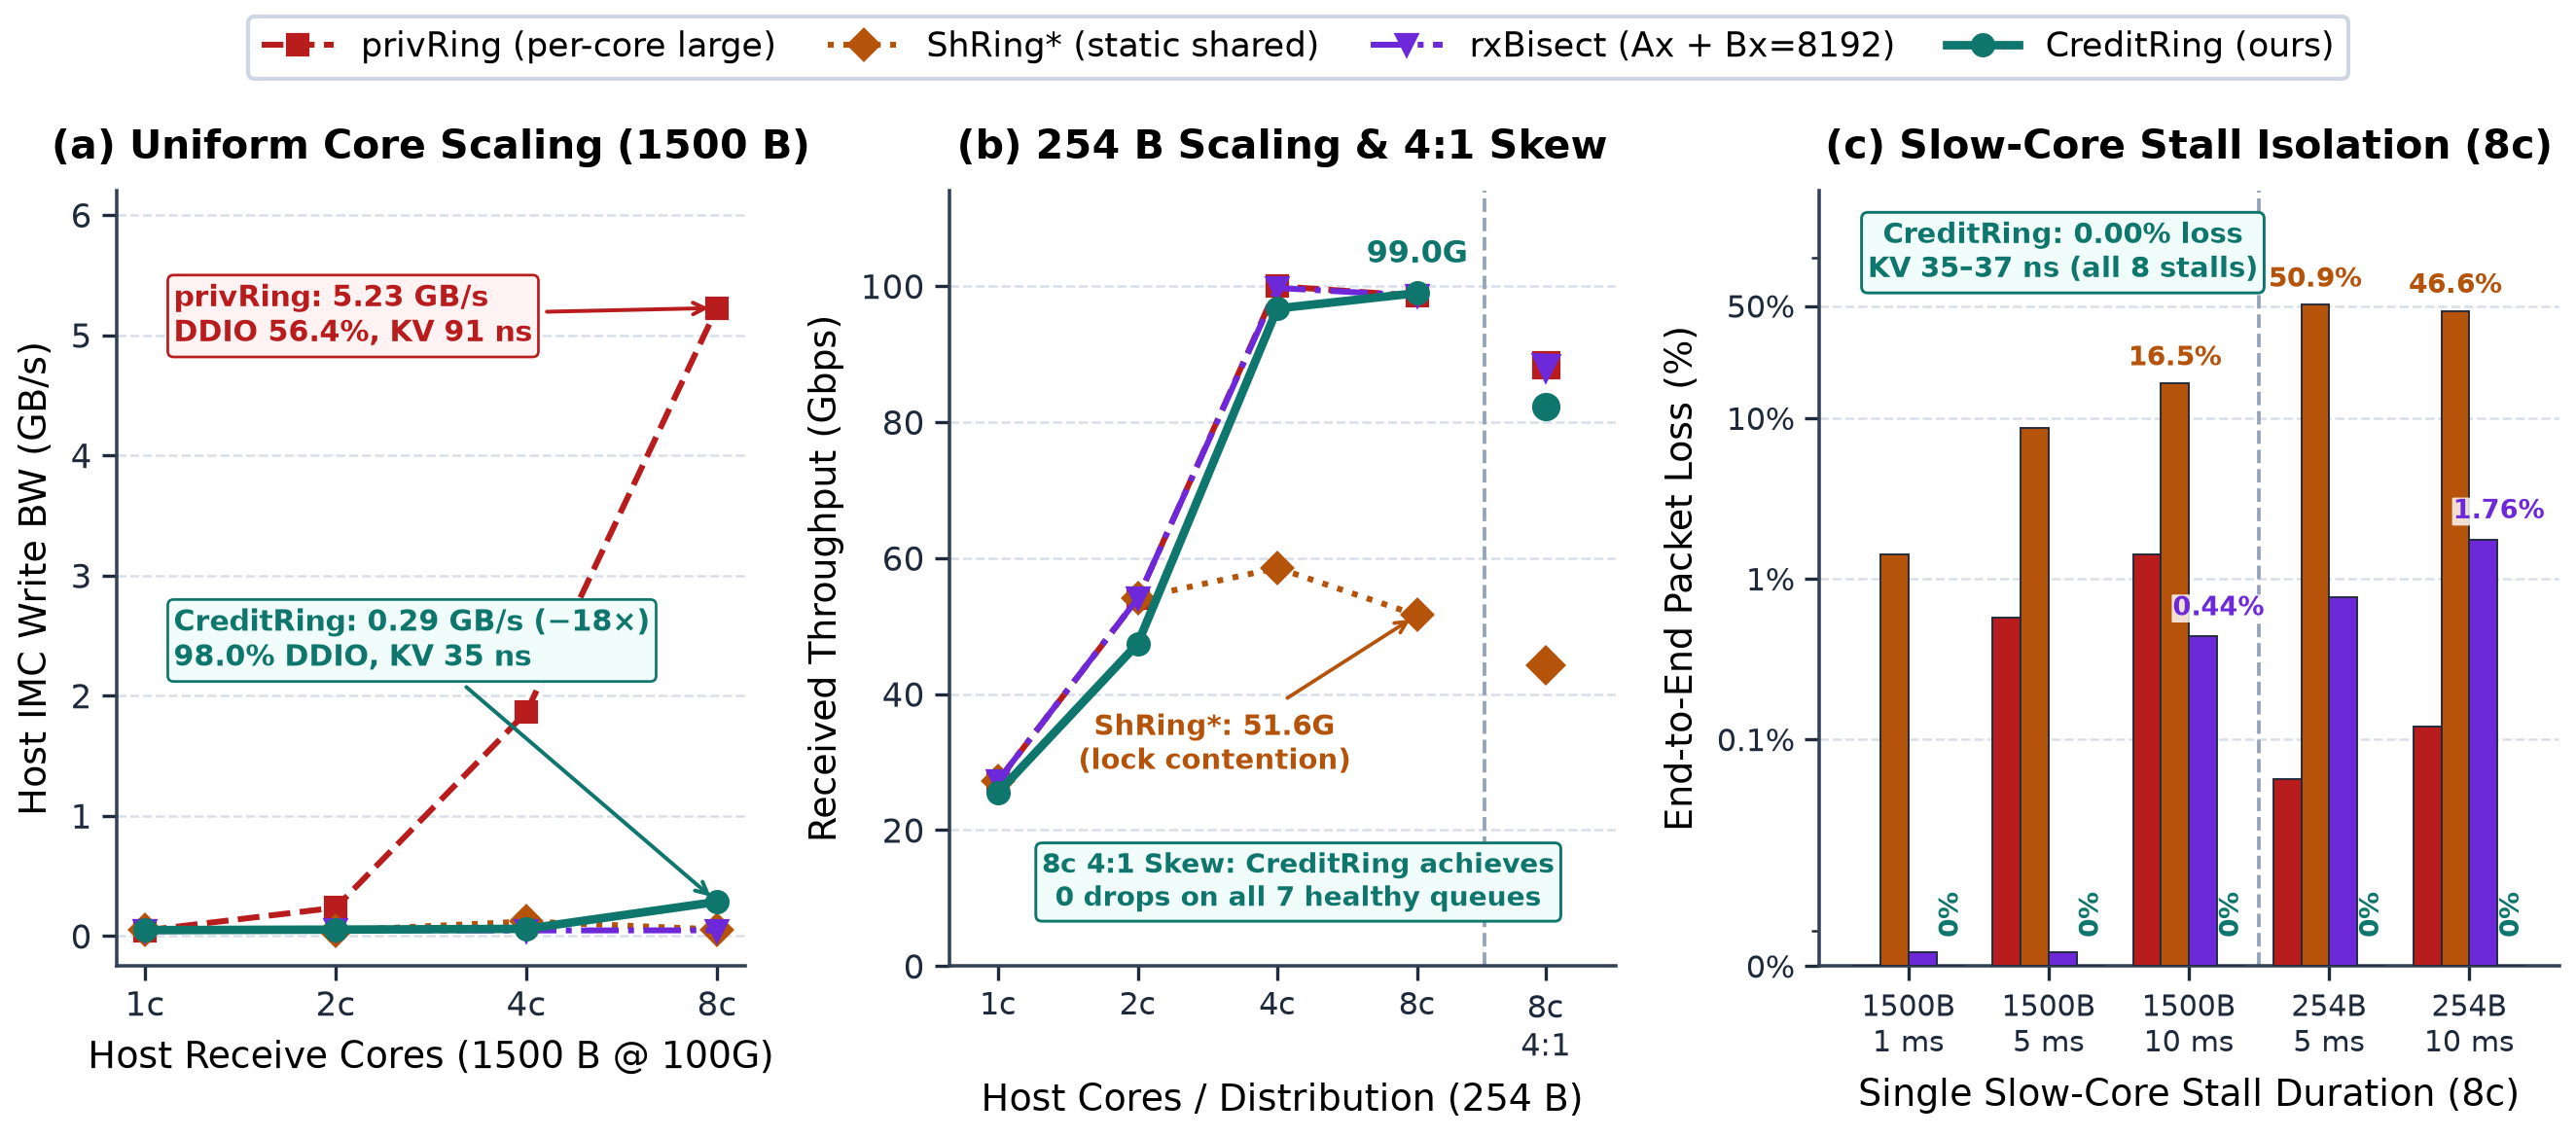
\includegraphics[width=\textwidth]{figures/fig4_e4_multicore.png}
  \caption{\textbf{E4 (291 runs, 11.9\,B pkts):} Multi-core comparison vs.\
  \texttt{privRing}, static \texttt{ShRing*}, and \texttt{rxBisect}.
  (a)~1$\to$8 cores (1500\,B): \texttt{privRing} blows DDIO (5.23\,GB/s IMC
  writes, KV $p99$ 91\,ns), while \sys{} stays 18$\times$ lower (0.29\,GB/s,
  98.0\% DDIO, KV 35\,ns). (b)~254\,B scales lock-free to 99.0\,Gbps vs.\
  \texttt{ShRing*} lock collapse (51.6\,Gbps), with 0 drops across all 7
  healthy queues under 4:1 skew. (c)~Under 1--10\,ms single-core stalls, only
  \sys{} sustains 0.00\% loss across all 8 configs with baseline 35--37\,ns KV.}
  \label{fig:e4}
\end{figure*}

Figure~\ref{fig:e4} evaluates 291 verified runs (11.91\,B packets) across 1--8
Socket~1 cores (\texttt{ism\_enable=0} uniformly) with a co-located 32\,MiB KV
neighbor (idle $p50=27$\,ns, $p99=35$\,ns, $p999=91$\,ns).

\paragraph{Uniform 1 $\to$ 8 core scaling.}
At 1500\,B 100GbE (Figure~\ref{fig:e4}(a)), scaling \texttt{privRing} to 8 cores
collapses DDIO from 100.0\% to 56.4\%, inflates host memory writes
\textbf{112$\times$} (0.05 $\to$ 5.23\,GB/s), and pushes KV LLC miss past a
deterministic \textbf{1.07\% physical step} into DRAM latency (\textbf{91\,ns}
median $p99$, $p999=143$\,ns): across all 291 runs, every run $<1.07\%$ miss
(263/263) stays $\le 43$\,ns, while every run $\ge 1.07\%$ (28/28) jumps to
$\ge 89$\,ns regardless of memory channel count. \sys{} reaches full
\textbf{100.1\,Gbps} at 8 cores with 0.00\% loss, 98.0\% DDIO, \textbf{0.29\,GB/s}
IMC writes (\textbf{18$\times$ lower}), and \textbf{35\,ns} KV $p99$.

On 254\,B (Figure~\ref{fig:e4}(b)), \sys{} scales lock-free to \textbf{99.0\,Gbps}
(45.16\,Mpps), matching \texttt{privRing}/\texttt{rxBisect} (98.6\,Gbps). All
three hit an 8-core \texttt{ism\_enable=0} synchronous register-read ceiling
($\sim$45.0--45.2 vs.\ 45.8\,Mpps offered), causing 1.46\% drops in
\texttt{privRing}/\texttt{rxBisect} and 1.05\% (718--777K) card FIFO overflow
in \sys{} once 3--4 queues fill 75K \texttt{mbuf}s ($\approx 173$\,MiB $>$
48\,MiB card L3). Static \texttt{ShRing*} drops to 51.6\,Gbps at 8 cores
(noting our prototype amplifies regular small-packet lock cost via double
locking per 32-pkt batch and \texttt{pool\_cache=32 < 64}; its decisive
architectural wall appears under stalls below).

\paragraph{RSS skew and 1--10\,ms slow-core stalls.}
Under 8-core 4:1 and Zipf skew (1500\,B), \sys{} keeps 98.8\% / 99.1\% DDIO,
0.00\% loss, and 18--21$\times$ lower IMC writes (0.18 / 0.17 vs.\ 3.80 /
3.05\,GB/s). On 254\,B 8-core 4:1 skew, \sys{} achieves strict \textbf{0 drops
on all 7 healthy queues} (vs.\ 125K \texttt{privRing}, 457K \texttt{rxBisect}
amplified by CN106's 256-slot non-backpressured ring, and 17.41M
\texttt{ShRing*}); sustained overload on hotspot \texttt{q0} lowers \texttt{q0}
by 25\% (8.36 vs.\ 11.22\,Mpps, total 82.3 vs.\ 88.4\,Gbps) because a
perpetually full 75K-\texttt{mbuf} FIFO (173\,MiB) overflows card L3 into
9.49\,GB/s card DDR5, motivating \texttt{CompactSlab} or $\le 16$K caps under
permanent overload.

Under periodic 1 / 5 / 10\,ms single-core stalls (Figure~\ref{fig:e4}(c);
1500\,B at 100GbE, 254\,B at 36\,Mpps / 79\,Gbps on 8c and 32\,Mpps on 4c),
static \texttt{ShRing*} suffers massive HoL drops (\textbf{1.42--16.49\%} on
1500\,B; \textbf{46.6--50.9\%} on 254\,B), while dynamic fallback to
\texttt{privRing} immediately forfeits DDIO. \texttt{rxBisect} avoids locks but
overflows $B_x=8192$, losing \textbf{70.5K--75.7K} (1500\,B, 0.44--0.52\%) and
\textbf{529K--1.24M} (254\,B, 0.77--1.92\%) packets (enlarging $B_x$ to 64K
would re-trigger host LLC eviction). \texttt{privRing} both drops up to 1.41\%
and blows DDIO (4.69--5.16\,GB/s IMC, KV $p99=95$\,ns / $p999=153$\,ns).
\textbf{\sys{}} achieves \textbf{0.00\% end-to-end loss across all 8 stall
configurations}, absorbing 982--10,216 (1500\,B) and 4,339--44,849 (254\,B)
packets in SmartNIC memory with 0 healthy-core drops, 20--24$\times$ lower host
IMC writes (0.20--0.25\,GB/s), and baseline \textbf{35--37\,ns} KV $p99$.

\subsection{E3: Head-to-Head Comparison vs.\ Dual-Path \ceio{}}
\label{sec:eval-e3}

\begin{figure*}[t]
  \centering
  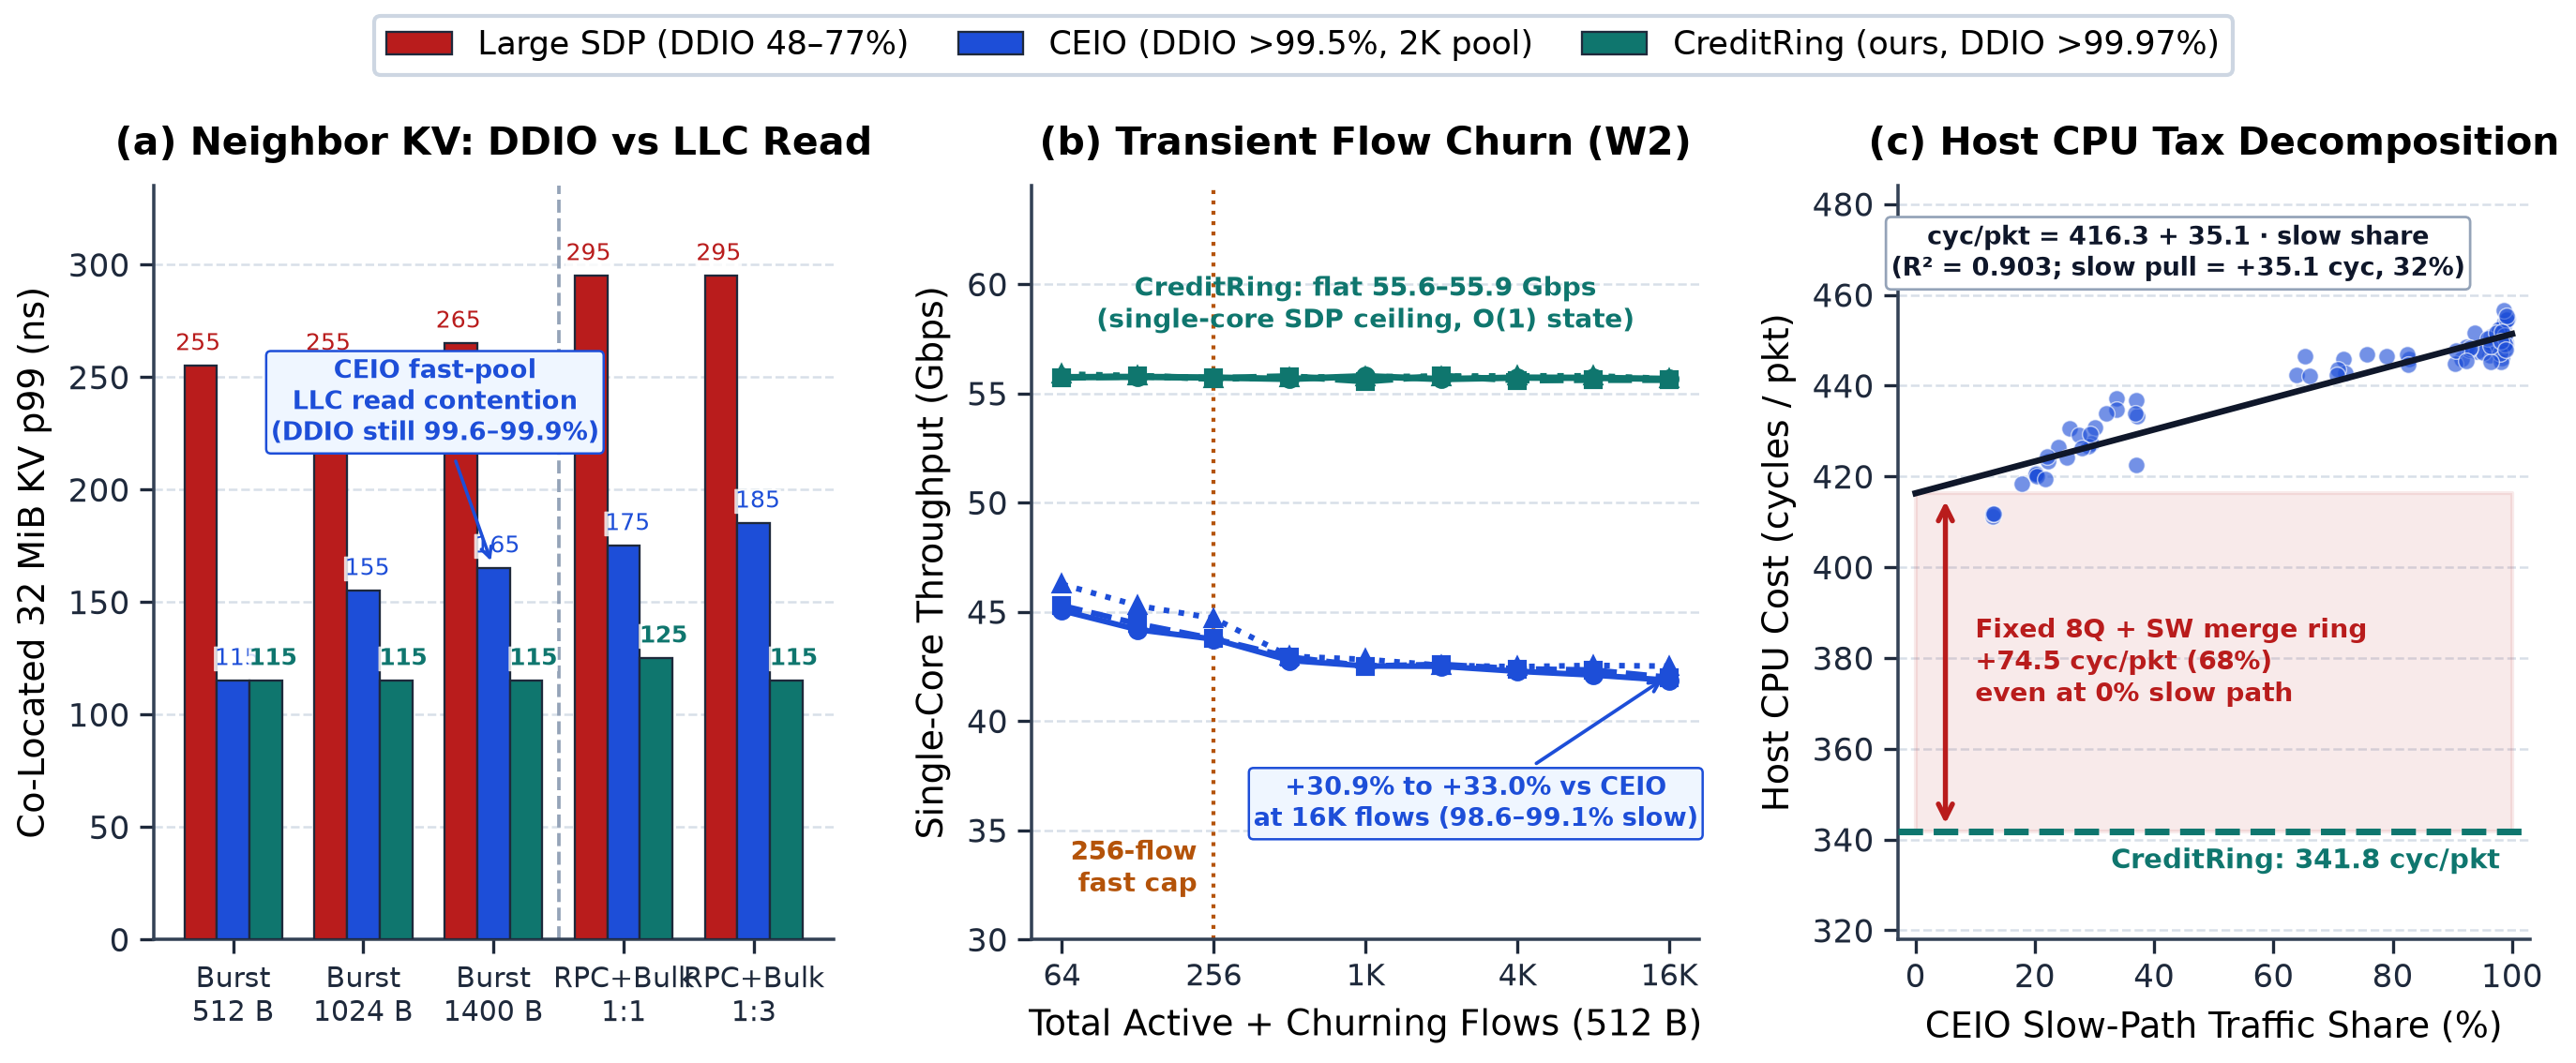
\includegraphics[width=\textwidth]{figures/fig5_e3_ceio_h2h.png}
  \caption{\textbf{E3 (240 runs):} Same-CN106 head-to-head vs.\ strengthened
  \ceio{} (equal 1,024-pkt host budget). (a)~Co-located KV $p99$ distinguishes
  \texttt{Large SDP}'s DDIO blowthrough (255--295\,ns) from \ceio{}'s 2048-slot
  fast-pool LLC read contention (155--185\,ns despite $>$99.5\% DDIO), while
  \sys{} holds 115--125\,ns. (b)~Across 64--16,384 churning flows, \sys{} holds
  flat at 55.6--55.9\,Gbps (+20.8--33.0\% over \ceio{}). (c)~Regression over 81
  \ceio{} runs proves 68\% (+74.5\,cyc/pkt) of \ceio{}'s CPU penalty is fixed
  at 0\% slow path from 8Q polling and 2P1C \texttt{SwMergeRing}.}
  \label{fig:e3}
\end{figure*}

Figure~\ref{fig:e3} compares \sys{}, strengthened \ceio{} (dedicated 5th control
core, 20\,$\mu$s credit flush, strict FIFO phase-hold), idealized zero-rewrite
\ceio{} (\texttt{ceio\_zero\_rmt}), and \texttt{Large SDP} across 240 verified
runs on identical hardware (single host core + co-located 32\,MiB KV neighbor).

\paragraph{Burst onset (W1) and LLC read-capacity contention.}
With 400\,$\mu$s pauses every 25\,ms across 512 / 1024 / 1400\,B frames, \sys{}
wins full-run $p99$ (\textbf{103.0 / 141.2 / 159.2\,$\mu$s}, $-$10.4--18.2\%
vs.\ \ceio{}, $-$7.3--9.9\% vs.\ \texttt{Large SDP}) and throughput
(\textbf{11.28 / 15.92 / 19.40\,Gbps}, +9.7--10.2\% vs.\ \ceio{}). (A higher
512\,B initial-500\,$\mu$s onset $p99$ median for \sys{} stems from a
+0.4\,ms/cycle post-pause timer beat precession rather than card queuing, which
affects $\le 0.04\%$ of onset packets.) Crucially, Figure~\ref{fig:e3}(a)
distinguishes two cache-interference mechanisms: \texttt{Large SDP} blows DDIO
(51.9--76.8\%, KV \textbf{255--265\,ns}), whereas \ceio{} preserves
\textbf{99.5--99.7\% DDIO} yet its 2048-slot fast-ring pools ($\sim$9--13.5\,MiB
rotating read footprint at 1024--1400\,B) contend with the 32\,MiB KV table for
60\,MiB shared LLC read capacity, inflating KV $p99$ to \textbf{155--165\,ns}
even with zero rule-rewrite latency (\texttt{ceio\_zero\_rmt}: 1400\,B
$p99=197.2\,\mu$s, KV 165\,ns). \sys{}'s 4\,MiB pool holds $>$99.97\% DDIO and
locks KV at \textbf{115\,ns}.

\paragraph{Transient flow churn (W2) and linear CPU decomposition.}
Across 64--16,384 churning flows (512\,B echo, 16 active flows rotating every
1\,ms / 500\,$\mu$s / 100\,$\mu$s, Figure~\ref{fig:e3}(b)), \sys{} stays flat
at the single-core SDP loopback ceiling (\textbf{55.6--55.9\,Gbps},
341.8\,cyc/pkt, $p99=98.5$--$99.5\,\mu$s; card-only echo is 100.0\,Gbps), while
\ceio{} drops from 45.1--46.3\,Gbps (64 flows) to 41.9--42.5\,Gbps past its
256-flow cap (98.6--99.1\% slow path, $p99=132.7$--$163.9\,\mu$s)---a
\textbf{+20.8--33.0\%} lead for \sys{}. Linear regression over all 81 \ceio{}
runs (Figure~\ref{fig:e3}(c)) yields
$\text{cyc/pkt} = 416.3 + 35.1 \cdot \text{slow\_frac}$ ($R^2 = 0.903$),
proving that \textbf{68\% (+74.5\,cyc/pkt, +167.4\,ins/pkt)} of \ceio{}'s CPU
overhead is fixed at 0\% slow path from 8-queue polling and 2P1C
\texttt{SwMergeRing}, with slow-path pulling adding +35.1\,cyc/pkt (32\%).
Because both \ceio{} paths traverse ARM cores on CN106 (producing a 7--8\% step
rather than BlueField-3's hardware-RMT cliff), this cleanly isolates host
dual-path tax that persists on any SmartNIC.

\paragraph{Mixed RPC + bulk (W3).}
Mixing 256\,B open-loop RPCs with 1400\,B bulk streams at balanced (1:1) and
heavy-burst (1:3) ratios, \sys{} achieves highest throughput (\textbf{87.0 /
90.0\,Gbps}, +10.4--10.8\% vs.\ \ceio{}, +11.5--16.3\% vs.\ \texttt{Large SDP}),
lowest RPC $p99$ (\textbf{86.3 / 88.0\,$\mu$s}, $-$8.4--8.5\% / $-$9.2--10.7\%),
100.00\% DDIO, and lowest KV $p99$ (\textbf{125 / 115\,ns} vs.\ 175--185 /
295\,ns). (Under light 3:1 load, \texttt{Large SDP} edges throughput 52.7 vs.\
51.4\,Gbps due to idle credit flushes while blowing DDIO to 70.8\% and KV to
285\,ns.) Because $W=1024 \le 4R_{\text{eff}}$, card priority queues never
engage (\texttt{queued\_hi == 0} in 18/18 runs), confirming that single-path
elimination alone delivers the full win.

\subsection{E5: Unmodified Memcached~1.6.45 and Stateful NFV}
\label{sec:eval-e5}

\begin{figure*}[t]
  \centering
  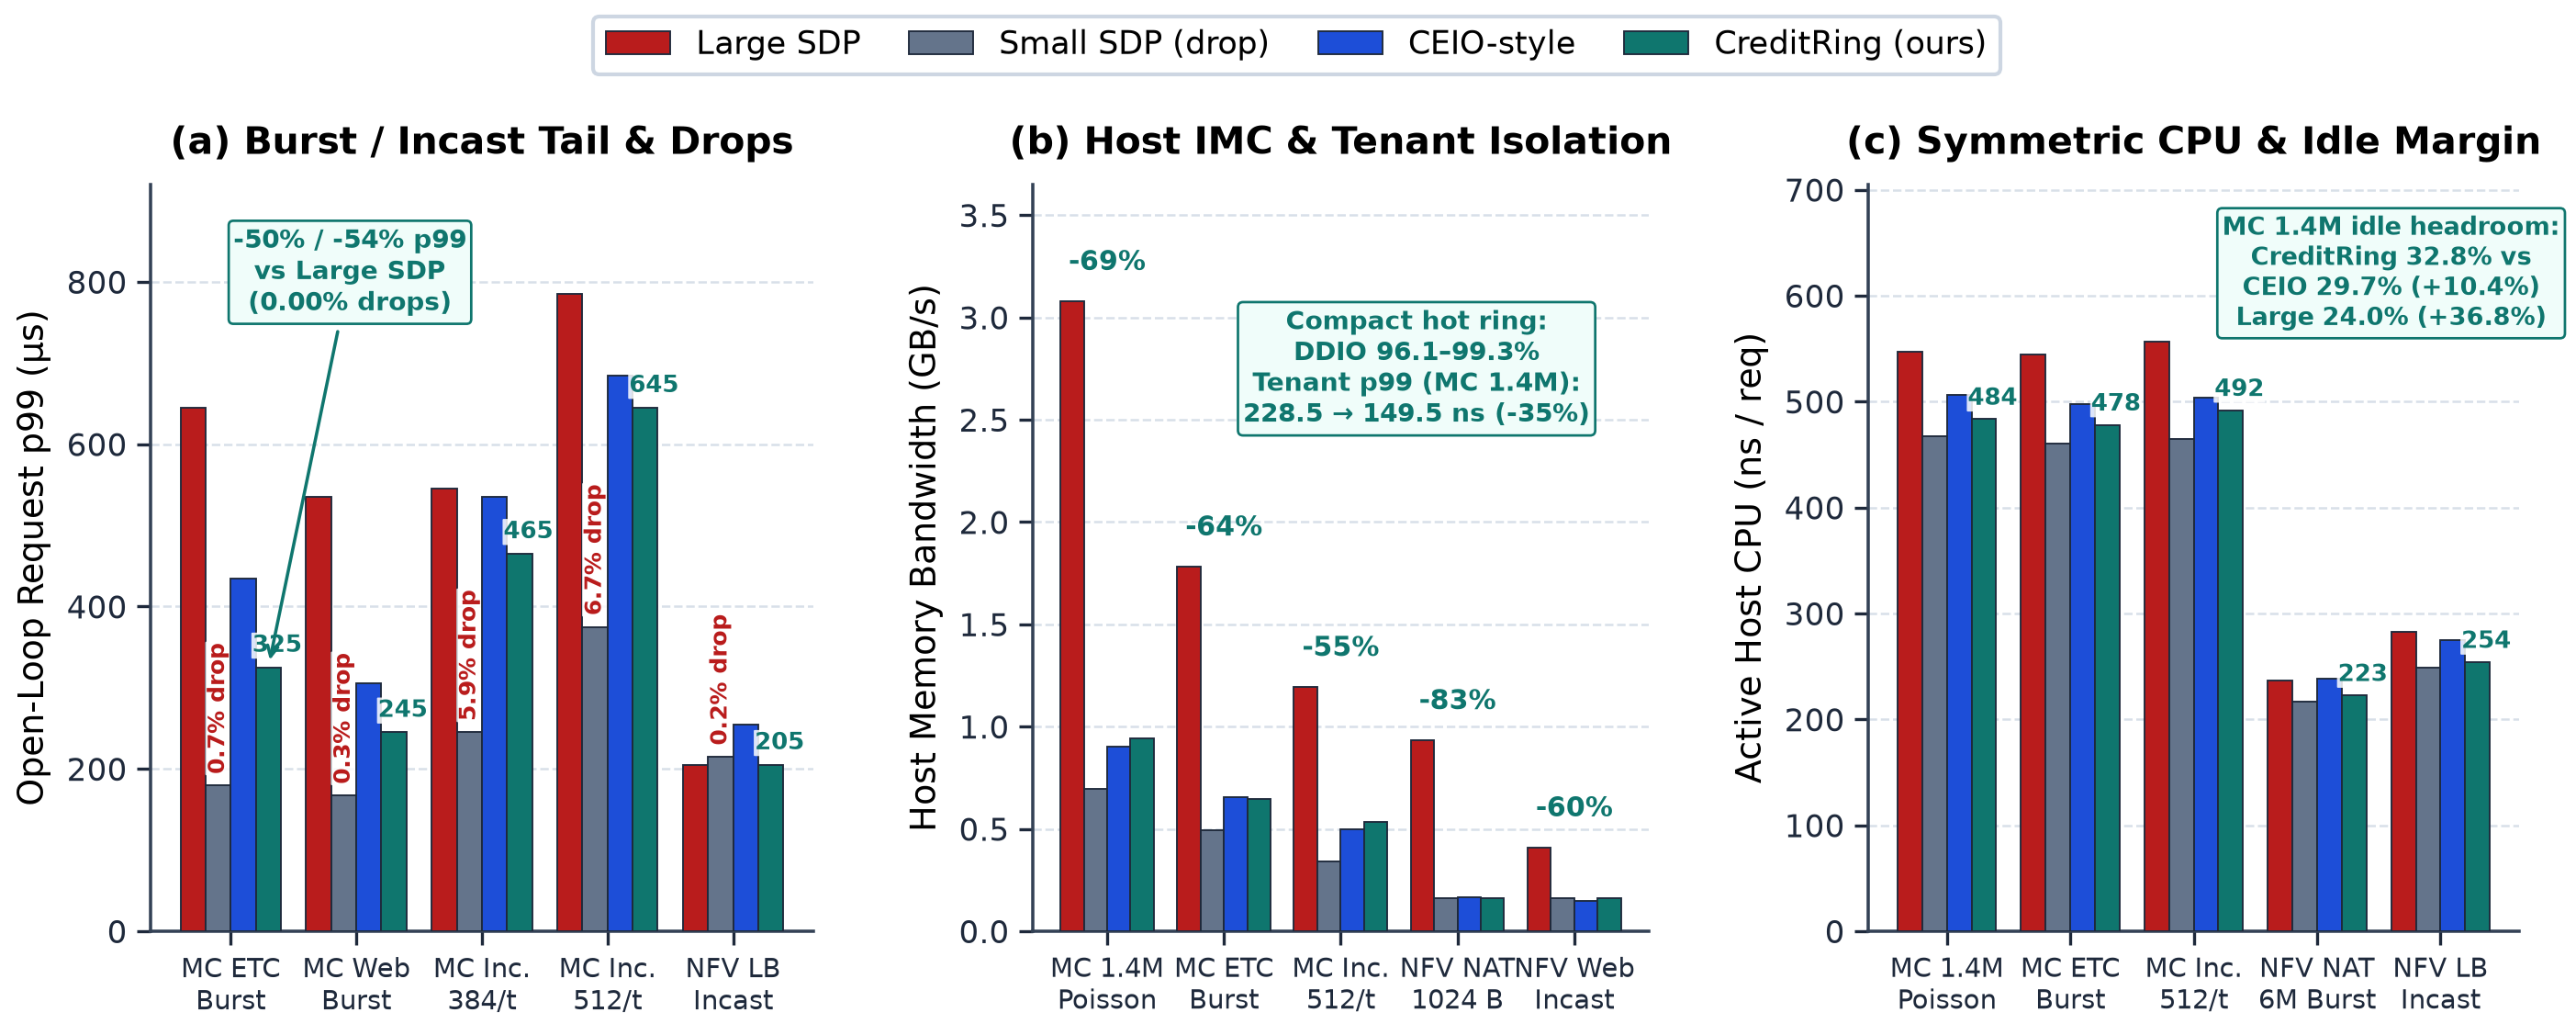
\includegraphics[width=\textwidth]{figures/fig6_e5_apps.png}
  \caption{\textbf{E5 (180 runs):} Unmodified upstream Memcached~1.6.45
  (\texttt{git diff = 0}) and 5-tuple stateful NFV over identical standard SDP
  rings with a co-located 32\,MiB tenant. (a)~Only \sys{} keeps 0.00\% drops
  while cutting Memcached microburst $p99$ by 50--54\% vs.\ \texttt{Large SDP}
  and 20--25\% vs.\ \texttt{CEIO-style}. (b)~Compact rings offload 55--83\%
  host memory bandwidth (64--83\% under high pressure) and cut MC 1.4M tenant
  $p99$ by 35\%. (c)~Symmetric per-(policy, app) \texttt{tau\_empty} CPU
  accounting confirms lowest host CPU and +10.4\% / +36.8\% higher real idle
  wall-clock headroom at 1.4M RPS.}
  \label{fig:e5}
\end{figure*}

Figure~\ref{fig:e5} and Table~\ref{tab:e5-summary} evaluate 180 verified runs
running unmodified upstream \textbf{Memcached~1.6.45}~\cite{fitzpatrick2004memcached}
(Facebook ETC~\cite{atikoglu2012memcached} and WebSearch~\cite{alizadeh2010dctcp})
and stateful 5-tuple \textbf{NFV} (NAT and Maglev LB~\cite{eisenbud2016maglev})
with a co-located 32\,MiB tenant on identical standard SDP rings.

\paragraph{Burst and incast performance.}
On Memcached microbursts (600k baseline + 1.5\,ms bursts at 3.5M RPS,
Figure~\ref{fig:e5}(a)), \texttt{Large SDP} drops DDIO to 82.0--83.2\% and
doubles Memcached's LLC misses (ETC 13.8\% vs.\ 5.9\%), inflating $p99$ to
\textbf{645 / 535\,$\mu$s}. \texttt{Small SDP} drops 0.69\% / 0.26\% on
microbursts and \textbf{5.82--6.70\%} on synchronized incast (1,536--2,048
packets/epoch), cutting goodput 15.6--18.0\%. \texttt{CEIO-style} leaks
104K--170.5K packets during its 25\,$\mu$s switch lag (overflowing to 0.01\%
drops at 512/thr incast), yielding 435 / 305\,$\mu$s microburst $p99$.
\textbf{\sys{}} achieves \textbf{0.00\% drops} across all 15 workloads, slashes
microburst $p99$ to \textbf{325 / 245\,$\mu$s} (\textbf{$-$49.6\% / $-$54.2\%}
vs.\ \texttt{Large SDP}, \textbf{$-$25.3\% / $-$19.7\%} vs.\ \texttt{CEIO-style}),
wins all three incast suites (465 / 645 / 445\,$\mu$s, $-$14.7--17.8\% vs.\
\texttt{Large SDP}), scales 256 $\to$ 4,096 flows with zero leakage (vs.\
1.70$\times$ leakage surge to 249.5K for \texttt{CEIO-style}), and adds zero
steady-state Poisson latency tax (15.2 / 18.5 / 22.1\,$\mu$s vs.\ 15.5 / 19.3 /
24.9\,$\mu$s; 1.4M $p999$ 31.4 vs.\ 72.8\,$\mu$s). On NFV, card queuing rarely
triggers (median depth 0), yet \texttt{CEIO-style} still worsens $p99$ by
+16--34\% (Maglev incast 255 vs.\ 205\,$\mu$s) because unconditional
\texttt{SwMergeRing} enqueueing + deferred TX adds $\sim$21\,ns/req
($+43\,\mu$s incast tail), whereas \sys{} stays lossless and matches or beats
\texttt{Large SDP}.

\begin{table*}[t]
\centering
\footnotesize
\setlength{\tabcolsep}{4.0pt}
\renewcommand{\arraystretch}{1.06}
\begin{tabular}{l l r r r r r r r r}
\toprule
\textbf{Workload (Standard SDP)} & \textbf{Policy} &
\textbf{Goodput} & \textbf{Drop} & \textbf{App $p99$} & \textbf{Tenant $p99$} &
\textbf{DDIO} & \textbf{Host IMC} & \textbf{Active CPU} & \textbf{Leak} \\
& & \textbf{(Mrps)} & \textbf{(\%)} & \textbf{($\mu$s)} & \textbf{(ns)} &
\textbf{(\%)} & \textbf{(GB/s)} & \textbf{(ns/req)} & \textbf{Pkts} \\
\midrule
MC ETC Microburst & \texttt{Large SDP}      & 0.772 & 0.00 & 645.0 & 144.5 & 83.2 & 1.78 & 544.3 & 0 \\
(600k/3.5M, 256f) & \texttt{Small SDP}      & 0.747 & 0.69 & 179.6 & 114.5 & 99.3 & 0.49 & 460.1 & 0 \\
                  & \texttt{CEIO-style}     & 0.772 & 0.00 & 435.0 & 114.5 & 98.6 & 0.66 & 497.9 & 146.8K \\
                  & \textbf{\sys{}}         & \textbf{0.772} & \textbf{0.00} & \textbf{325.0} & \textbf{115.5} & \textbf{98.6} & \textbf{0.65} & \textbf{478.1} & \textbf{0} \\
\midrule
MC WebSearch Burst & \texttt{Large SDP}     & 0.772 & 0.00 & 535.0 & 128.5 & 82.0 & 1.36 & 527.0 & 0 \\
(600k/3.5M, 256f)  & \texttt{Small SDP}     & 0.762 & 0.26 & 167.2 & 113.5 & 99.2 & 0.41 & 446.4 & 0 \\
                   & \texttt{CEIO-style}    & 0.773 & 0.00 & 305.0 & 113.5 & 98.5 & 0.51 & 479.0 & 104.0K \\
                   & \textbf{\sys{}}        & \textbf{0.773} & \textbf{0.00} & \textbf{245.0} & \textbf{113.5} & \textbf{98.5} & \textbf{0.50} & \textbf{461.8} & \textbf{0} \\
\midrule
MC ETC Incast      & \texttt{Large SDP}     & 0.482 & 0.00 & 785.0 & 114.5 & 80.8 & 1.19 & 556.5 & 0 \\
(512/thr, 1024f)   & \texttt{Small SDP}     & 0.395 & 6.70 & 375.0 & 106.5 & 99.0 & 0.34 & 464.7 & 0 \\
                   & \texttt{CEIO-style}    & 0.482 & 0.01 & 685.0 & 111.5 & 98.2 & 0.50 & 503.6 & 170.5K \\
                   & \textbf{\sys{}}        & \textbf{0.481} & \textbf{0.00} & \textbf{645.0} & \textbf{112.5} & \textbf{98.1} & \textbf{0.53} & \textbf{491.9} & \textbf{0} \\
\midrule
MC ETC Steady      & \texttt{Large SDP}     & 1.400 & 0.00 & 24.9  & 228.5 & 86.2 & 3.08 & 547.1 & 0 \\
(1.4M Poisson)     & \texttt{CEIO-style}    & 1.400 & 0.00 & 23.1  & 147.5 & 99.3 & 0.90 & 506.4 & 0 \\
                   & \textbf{\sys{}}        & \textbf{1.400} & \textbf{0.00} & \textbf{22.1} & \textbf{149.5} & \textbf{99.3} & \textbf{0.94} & \textbf{483.5} & \textbf{0} \\
\midrule
NFV Maglev Incast  & \texttt{Large SDP}     & 0.882 & 0.00 & 205.0 & 110.5 & 85.3 & 0.33 & 282.3 & 0 \\
(512/thr, 512f)    & \texttt{Small SDP}     & 0.870 & 0.24 & 215.0 & 50.5  & 99.7 & 0.12 & 248.5 & 0 \\
                   & \texttt{CEIO-style}    & 0.882 & 0.00 & 255.0 & 97.5  & 99.6 & 0.14 & 274.9 & 0 \\
                   & \textbf{\sys{}}        & \textbf{0.882} & \textbf{0.00} & \textbf{205.0} & \textbf{100.5} & \textbf{99.6} & \textbf{0.13} & \textbf{254.0} & \textbf{0} \\
\bottomrule
\end{tabular}
\caption{Selected \textbf{E5 (180 runs)} results on unmodified Memcached~1.6.45
and stateful NFV over identical standard SDP rings ($n=3$ medians; active CPU
via symmetric independent \texttt{tau\_empty} calibration).}
\label{tab:e5-summary}
\end{table*}

\paragraph{Causal attribution and symmetric CPU accounting.}
Figure~\ref{fig:e5}(b) confirms clean causality: all three compact-ring
policies yield similar DDIO (96.1--99.8\% vs.\ 40.9--90.2\%), host IMC offload
(\textbf{64--83\%} on high-pressure workloads, \textbf{55--83\%} across all
medium/heavy/burst runs, 35--53\% on light steady load near the 0.11\,GB/s
tenant floor), and tenant $p99$ relief (MC 1.4M: 228.5 $\to$ 149.5\,ns, $-34.6\%$;
MC burst: 144.5 $\to$ 115.5\,ns; NFV 6M: 111.5 $\to$ 52.5\,ns, $-52.9\%$).
(At light NFV 500k--1.5M, the 4\,KiB-page tenant's 0.707\% solo LLC miss sits
near the 1\% $p99$ cliff, causing minor page-coloring variation across compact
runs while $p95$ holds at 47.5\,ns and $p999$ stays well below \texttt{Large SDP}.)
Thus, the compact hot ring creates cache offload while \sys{} uniquely makes it
lossless under bursts. Using independent per-\texttt{(policy, app)} empty-poll
calibration $\tau_{\text{empty}}$ ($R^2 = 0.990$--$0.99998$, 84.4--88.0\,ns/poll,
Figure~\ref{fig:e5}(c)) to remove timing-instrumentation asymmetry, \sys{} cuts
active host CPU by \textbf{$-$5.8--13.5\%} vs.\ \texttt{Large SDP} and
\textbf{$-$1.7--9.3\%} vs.\ \texttt{CEIO-style} (only +4--6\,ns/req over bare
dropping \texttt{Small SDP} on NFV), preserving \textbf{32.8\%} real idle
wall-clock headroom at MC 1.4M---\textbf{+10.4\%} more than \texttt{CEIO-style}
(29.7\%) and \textbf{+36.8\%} more than \texttt{Large SDP} (24.0\%).

\subsection{E6: Design-Space Sensitivity and Guidelines}
\label{sec:eval-e6}

\begin{figure*}[t]
  \centering
  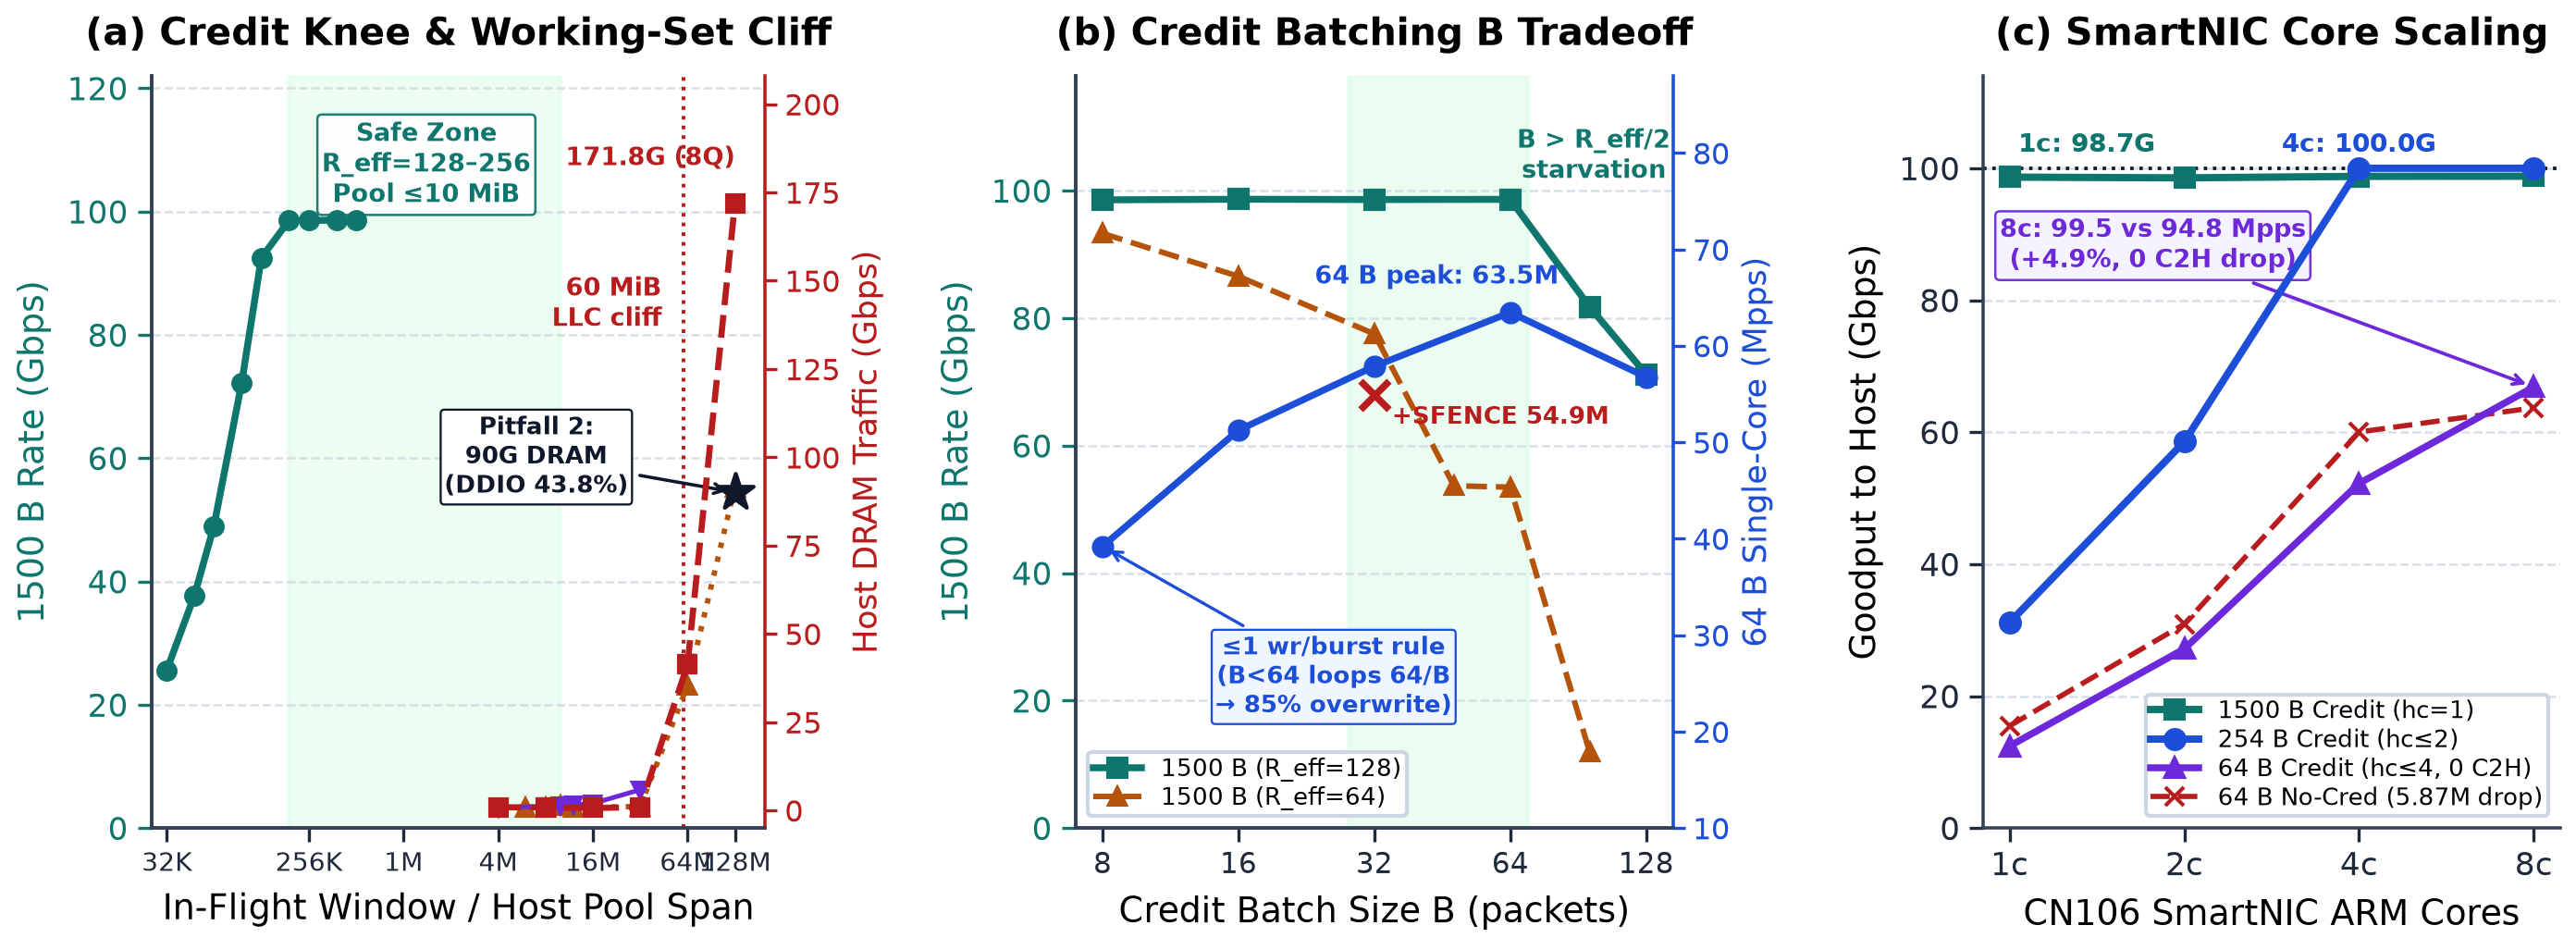
\includegraphics[width=\textwidth]{figures/fig7_e6_guidelines.png}
  \caption{\textbf{E6 (265 runs, 87 configs):} Operational design guidelines
  (\texttt{ism\_enable=0}). (a)~Left BDP knee clears at $R_{\text{eff}} \ge 96$
  (1500\,B); right sweep exposes Pitfall~2 ($R_{\text{eff}}=256$ + 128\,MiB
  pool $\to$ 90.1\,Gbps DRAM, 43.8\% DDIO) and the 60\,MiB full-LLC cliff
  (171.8\,Gbps at 8Q$\times$128\,MiB), defining $R_{\text{eff}}=128$--$256$ +
  pool $\le 10$\,MiB. (b)~Batching peaks at $B=64$ (63.5\,Mpps on 64\,B), obeys
  $B \le R_{\text{eff}}/2$ on 1500\,B, and validates the $\le$1 write/burst
  rule. (c)~1, 4, and 8 CN106 cores cover 1500\,B (98.7G), 254\,B (100.0G), and
  64\,B (99.5\,Mpps, 0 C2H drops, +4.9\% over credit-off).}
  \label{fig:e6}
\end{figure*}

Figure~\ref{fig:e6} synthesizes 265 verified sensitivity runs (all 219
credit-ring runs strictly 0 C2H drops) into three deployment rules:
\begin{enumerate}
\item \textbf{Keep $R_{\text{eff}}=128$--$256$/queue and aggregate hot pool $\le 10$\,MiB
  (Figure~\ref{fig:e6}(a)).} Under conservative \texttt{ism\_enable=0} polling
  (effective RTT 7.6--8.4\,$\mu$s), 1500\,B clears its BDP knee at
  $R_{\text{eff}} \ge 96$ (\textbf{98.5--98.7\,Gbps}, including $D=256,
  R_{\text{eff}}=128$). Pools $\le 10$\,MiB ($\le 7.5$\,MiB real 1500\,B write
  footprint) hold \textbf{99.7--100.0\%} DDIO (0.29--0.62\,Gbps IMC write). On
  an \emph{idle} single-queue socket, sequential L2 prefetching lifts 12--32\,MiB
  header-only rings into general LLC (94.8\% DDIO at 32\,MiB, though 8-queue
  splitting breaks prefetching and drops DDIO to 88.8--95.7\% even at 9\,MiB),
  while full-touch runs hit a hard \textbf{60\,MiB full-LLC cliff} (35.3\,Gbps
  1Q 64\,MiB, 91.6\,Gbps 1Q 128\,MiB, \textbf{171.8\,Gbps} 8Q 128\,MiB / 40.3\%
  DDIO). Pairing $R_{\text{eff}}=256$ with a 128\,MiB FIFO pool (\emph{Pitfall~2})
  still crashes DDIO to \textbf{43.8\%} (90.1\,Gbps DRAM).
\item \textbf{Set $B=32$--$64$ ($\le R_{\text{eff}}/2$) with $\le 1$ write per
  receive burst (Figure~\ref{fig:e6}(b)).} On 1500\,B, $R_{\text{eff}}=128$
  holds 98.6\,Gbps for $B \le 64$ (reverse PCIe write 0.13--0.19\,Gbps,
  $<0.2\%$ of link) and starves past $R_{\text{eff}}/2$ ($B=96 \to 81.7$\,Gbps;
  $R_{\text{eff}}=64, B=96 \to 11.9$\,Gbps). On 64\,B single-core saturation
  ($R_{\text{eff}}=256$, fixed 64-pkt bursts), rate peaks at \textbf{$B=64$
  (63.46\,Mpps, 61.2\,cyc/pkt, 2.79\% SB stalls)} vs.\ 57.89\,Mpps at $B=32$
  (+SFENCE cuts $B=32$ to 54.93\,Mpps; credit-off reaches 80.95\,Mpps only by
  silently dropping 10.83M packets, 7.89\%). Looping $64/B$ writes to the same
  BAR4 line at $B=8$ (39.21\,Mpps, +2,413\,cyc/64p) wastes 85\% via overwrite
  and incurs 75\% non-SB mesh/MMIO serialization (whereas 1500\,B without
  looping stays flat at 479--481\,cyc/pkt across $B=8$--$128$).
\item \textbf{Provision 1 / 4 / 8 SmartNIC cores for 1500\,B / 254\,B / 64\,B
  (Figure~\ref{fig:e6}(c)).} On CN106, \textbf{1 card core} saturates 100GbE at
  1500\,B (\textbf{98.7\,Gbps}, $h_c=1$) and \textbf{4 cores} saturate 254\,B
  (\textbf{100.0\,Gbps}, 45.62\,Mpps, $h_c=2$). On 64\,B 148.8\,Mpps overload
  ($h_c \le 4$), 1--4 cores scale 4.20$\times$ (18.49 $\to$ 77.71\,Mpps) and
  \textbf{8 cores} deliver \textbf{99.48\,Mpps} (66.9\,Gbps) with \textbf{0 C2H
  drops}---\textbf{+4.9\% above credit-off} (94.79\,Mpps, 5.87M silent host
  drops) by cleanly shedding excess at the card ingress FIFO before PCIe.
\end{enumerate}
